\newcommand{\drawNaivePricingFigure}{
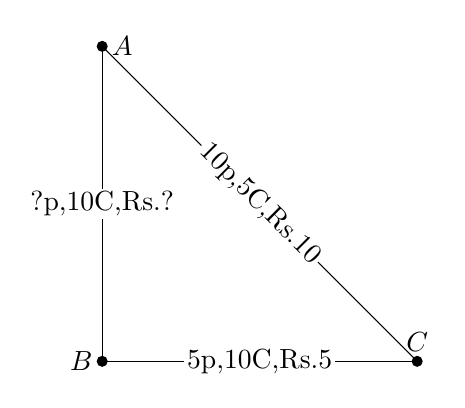
\begin{tikzpicture}
    % Define coordinates for the three nodes A, B, and C
    \coordinate (A) at (0, 4);
    \coordinate (B) at (0, 0);
    \coordinate (C) at (4, 0);

    % Draw the edges and label them using the 'midway' option
    % Edge A -- B
    \draw (A) -- (B) node [midway, fill=white, inner sep=1pt] {?p,10C,Rs.?};

    % Edge A -- C
    \draw (A) -- (C) node [midway, fill=white, inner sep=1pt, sloped] {10p,5C,Rs.10};

    % Edge B -- C
    \draw (B) -- (C) node [midway, fill=white, inner sep=1pt, sloped] {5p,10C,Rs.5};

    % Draw and label the vertices (Nodes)
    \fill (A) circle (2pt) node [right] {$A$};
    \fill (B) circle (2pt) node [left] {$B$};
    \fill (C) circle (2pt) node [above] {$C$};

\end{tikzpicture}
}